\begin{recipe}
    [% 
        preparationtime = {\unit[15]{min}},
        portion = {\portion{4}},
        bakingtime = {\unit[30]{min}}
    ]
    {Rhubarb crumble}

    \introduction{%
        There are three reasons why I love crumbles: preparation is super quick;
        no wheat; little sugar yet is very sweet due to fruit.
    }

    \ingredients{%
        600-800 g & Rhubarb \\
        5 & Apricots \\
        2 hfl. & Berries \\
        2 hfl. & Blueberries (fresh or frozen) \\
        & \\
        100 g. & Butter \\
        \nicefrac{1}{2} c. & Sugar \\
        1~\nicefrac{1}{2} c. & Oat flakes \\
        3 tbs. & Coconut milk powder \\
        1 tbs. & Ginger \\
        \nicefrac{1}{4} ts. & Salt
    }

    \preparation{%
        \step Cut rhubarb into 2-3 cm long pieces, apricots into quarters.
        Mix with berries in an oven dish/tin.


        \step In a hand blender s-shaped knife container (or using your hands) mix all ingredients for crumble topping.
        Add more fat/oats if needed


        \step Cover fruit with crumble topping. \underline{Bake at}
        \underline{\unit[180-200]{\textcelcius} for 20-30 min} till brown.
    }

    \hint{%
        Serve with ice cream or clotted cream.
    }

\end{recipe}


\begin{figure}[h]
    \centering
    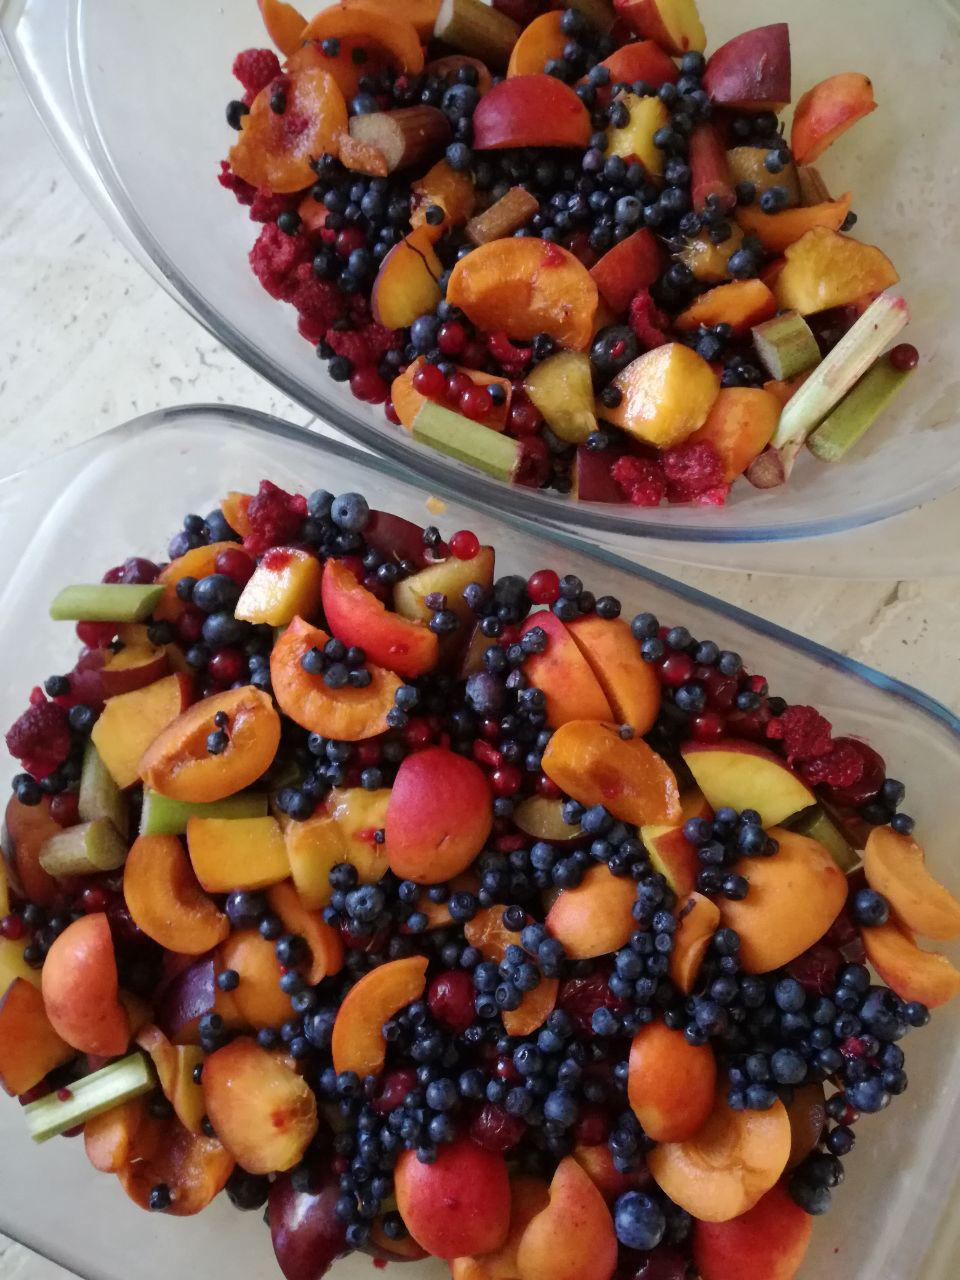
\includegraphics[width=8cm]{pic/crumble}
\end{figure}
